\section{Testing and Demonstration}
\label{sec:test}

Testing moved from host code to emulated hardware, then to the bench, and
finally to the water, so that each layer was checked before the next depended
on it. Table~\ref{tab:tests} summarizes the tests and their outcomes.

\subsection{Unit Tests}
The route manager, geometry library, and tack planner are compiled with the host C compiler
and exercised by a test harness: CRC values, waypoint validation, incomplete
and corrupted uploads, angle wrapping, bearings, track distances, and circular
means. The tack planner adds tests for every state transition, corridor
and layline tacks, arrival, stale inputs, and wind wrap-around. On the
\texttt{ltp} branch (commit \texttt{ca2e48e}), all 1275 checks pass: 68
geometry, 266 route, and 941 tack-planner checks.

\subsection{Firmware-in-the-Loop Simulation}
Fig.~\ref{fig:sim} shows the simulator the team built to develop control
logic before water time was available. The unmodified CM7 firmware runs on an
emulated STM32H755 in the Renode framework~\cite{renode}. Each sensor is
emulated at the bus level: BNO055 and AS5600 registers over
I\textsuperscript{2}C, the wind vane's Modbus replies over UART, and NMEA
sentences from the GPS. The real drivers therefore run without changes. A
lockstep bridge passes the firmware's servo pulse widths to a Python physics
model of the boat, which returns sensor values. The model is built from the
CAD exports. It takes wing, tail, keel, and rudder areas and the pivot
locations from the geometry, computes buoyancy and righting moment from a
voxel model of the hull and keel, and takes mass and center of gravity from an
editable mass list. It adds wind gusts and shifts, water current, wind-vane
position effects, sensor noise, and the $\pm\SI{90}{\degree}$ wing stops. A
browser dashboard shows the boat in 3D and provides tabs for live sailing,
a bench setup with a fan, route planning, stability curves, and a
points-of-sail polar. Sensors can be failed on command to test the fallback
logic.

The simulator does not yet emulate the CM4 or the radio. Heel is
quasi-static, and hull drag and the tail-to-angle-of-attack gain are estimates
to be calibrated from water tests. It is therefore used to develop and
debug logic, while gains are tuned on the water.

\begin{figure}[!t]
\centering
\begin{tikzpicture}[font=\scriptsize, >={Stealth[length=2mm]},
  bx/.style={draw, rounded corners=2pt, align=center, minimum width=28mm, minimum height=9mm}]
\node[bx, fill=blue!6, minimum height=24mm] (ren) at (0,0) {\textbf{Renode}\\emulated STM32H755\\unmodified CM7 firmware\\[3pt]sensor models:\\BNO055, AS5600\\wind vane, GPS};
\node[bx, fill=gray!12, minimum height=24mm] (pl) at (4.6,0) {\textbf{Physics plant}\\(Python)\\[3pt]hull, keel, rudder\\wing and tail\\hydrostatics\\wind and current\\noise and faults};
\node[bx, fill=green!8] (dash) at (4.6,2.35) {Browser dashboard\\3D view, controls, charts};
\draw[->] ([yshift=4mm]ren.east) -- node[above]{servo PWM} node[below,font=\tiny]{lockstep} ([yshift=4mm]pl.west);
\draw[<-] ([yshift=-4mm]ren.east) -- node[below]{sensor values} ([yshift=-4mm]pl.west);
\draw[<->] (dash) -- (pl);
\node[bx, fill=orange!10] (cad) at (0,2.35) {CAD exports (STL)\\and mass list};
\draw[->] (cad) -- (dash.west);
\end{tikzpicture}
\caption{Firmware-in-the-loop simulator. The flight firmware runs unchanged on
an emulated microcontroller and sails a physics model built from the CAD.}
\label{fig:sim}
\end{figure}

\subsection{Bench Tests}
The firmware includes several bench tools that are compiled in only when
needed. A serial console on the ST-LINK USB port, together with a host script
that works with both the real and the emulated board, moves each servo, sweeps
it through its range, and reports status. A dummy-telemetry mode transmits a
fixed packet of recognizable values so that decoding at the ground station
can be checked by eye. A fake-command mode feeds a scripted command list
through the same parse path as received packets, and a commander self-test
steps through every mode at boot. A command stress test sends a long burst
of commands through the inter-core ring. A debug console reports each task's
remaining stack and the share of time the RTOS spends busy, and a fault handler
reports the cause and location of a crash over the serial port. These tools found several faults before the boat reached the water.
\begin{itemize}
\item \emph{Servos.} Both servos map $\pm\SI{90}{\degree}$ to 500 to
\SI{2500}{\micro\second} pulses, centered at \SI{1500}{\micro\second}, and
the arbiters clamp each command to that range. Before the field test, the
team found and fixed a fault in which the rudder arbiter reversed the
commanded direction; on the water, the rudder then followed manual commands
from $+80$ to $-\SI{70}{\degree}$.
\item \emph{Sensors.} Each driver was brought up on the bench before
integration. The sail-angle encoder's range check compared raw counts
against \SI{360}{\degree} and rejected valid readings until it was
corrected. The battery taps were moved off pin PA1, which the Nucleo
board ties to the Ethernet clock (Section~\ref{sec:elec}).
\item \emph{Radio link.} Telemetry first failed to reach the ground
station because the sensor polling tasks starved the telemetry task, so no
packet was ever copied into shared memory. Raising the telemetry task's
priority fixed it. A second fault on the CM4 discarded received commands
whenever a packet was sent, which was fixed by handling reception before
transmission. The half-duplex timing window described in
Section~\ref{sec:sw} was also measured on the bench.
\end{itemize}

\subsection{Field Test}
\label{sec:field}
The first on-water test took place on November 18, 2026, from 16:02 to 16:25,
on Decker Lake pond in the Salt Lake Valley. The operator steered by
sending heading targets in SEMI\_RUDDER\_AUTO\_SAIL mode, so the heading PID,
sail planner, and sail PID were all closed-loop, and finished with manual
rudder in AUTO\_SAIL\_MAN\_RUDDER. The tack planner was not on board.
The link-loss timeout was disabled; it is compiled out on both \texttt{master}
and \texttt{ltp}. The firmware from \texttt{master} was used for this test. Every packet was logged at the ground station. The wind came from
about \SI{294}{\degree} (west-northwest), taken as the circular mean of
heading plus apparent wind angle over the water portion. Wind speed was not
measured on board; the National Oceanic and Atmospheric Administration (NOAA) wind report gave gusts of up to \SI{15}{mph}
(\SI{6.7}{\meter\per\second}), and the water was calm.

Fig.~\ref{fig:field_track} shows the track. From 16:02 to 16:09 the boat
was wheeled to the launch point on its cart, so the track follows the
shoreline footpath and the IMU shows almost no roll. After launch at about 16:09:30, the boat spent
\SI{15.9}{\minute} on the water. It covered \SI{375}{\meter} along its track
and reached \SI{228}{\meter} from the launch point, at a median speed of
\SI{0.35}{\meter\per\second} (peak \SI{0.77}{\meter\per\second}) over
30-second windows.

\begin{figure}[!t]
\centering
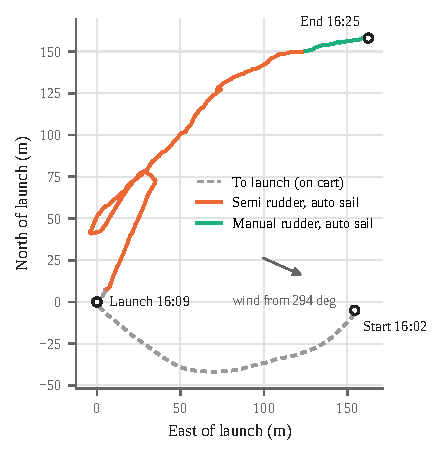
\includegraphics[width=\columnwidth]{field_track}
\caption{GPS track from the November 18 field test, in meters from the launch
point. The dashed segment is the walk to the launch point on the cart; the boat
sailed the solid segments, first with heading targets (semi rudder) and then
with manual rudder, with the sail on auto throughout.}
\label{fig:field_track}
\end{figure}

\paragraph*{Heading control}
Fig.~\ref{fig:field_heading} shows the heading, its target, and the rudder
angle, and Table~\ref{tab:field_heading} summarizes each target held for
longer than \SI{20}{\second}. Error statistics exclude the first
\SI{20}{\second} after each new target. Three behaviors stand out.
\begin{enumerate}
\item On every target at least \SI{49}{\degree} from the wind, the heading
PID held the target with a mean absolute error (MAE) of 3.8 to \SI{8.2}{\degree},
and the rudder was at its \SI{35}{\degree} limit no more than 12\% of the
time.
\item On the two targets inside the no-go zone (\SI{290}{\degree} and
\SI{302}{\degree}, within \SI{6}{\degree} of the wind), the boat settled 42 to
\SI{46}{\degree} off the wind with the rudder at its limit about 90\% of the
time. This measures the boat's closest pointing angle, and it agrees with the
\SI{45}{\degree} no-go angle assumed by the tack planner.
\item At 16:16:50 the boat, on a heading of about \SI{240}{\degree}, was
given a target of \SI{20}{\degree}. The heading PID turns the short way,
which here was through the wind, and the boat stalled in irons for two
minutes with the rudder at its limit. The heading PID alone cannot tack; the
planner's TACKING state, which turns only between close-hauled headings on
each side, exists for exactly this case. A later target of \SI{150}{\degree},
which required bearing away by about \SI{105}{\degree}, was also not reached
in the \SI{27}{\second} before the next command, despite full rudder.
\end{enumerate}

\begin{table}[!t]
\caption{Heading Hold in the Field Test (Wind from About 294$^\circ$)}
\label{tab:field_heading}
\centering
\footnotesize
\begin{tabular}{@{}lrrrrr@{}}
\toprule
Start & Target & Off wind & Held & MAE & Rudder at \\
      & (deg)  & (deg)    & (s)  & (deg) & limit \\
\midrule
16:10:22 & 200 & 90  & 111 & 5.7   & 0\% \\
16:12:26 & 20  & 83  & 90  & 3.8   & 2\% \\
16:14:06 & 200 & 93  & 25  & 4.4   & 12\% \\
16:14:32 & 245 & 49  & 78  & 8.2   & 1\% \\
16:15:50 & 290 & 6   & 32  & 37.5  & 88\% \\
16:16:23 & 200 & 91  & 26  & 22.4  & 44\% \\
16:16:50 & 20  & 97  & 122 & 142.4 & 99\% \\
16:18:53 & 200 & 98  & 44  & 65.2  & 50\% \\
16:19:38 & 150 & 160 & 27  & 108.8 & 100\% \\
16:20:06 & 302 & 2   & 131 & 43.5  & 90\% \\
\bottomrule
\end{tabular}
\end{table}

\begin{figure}[!t]
\centering
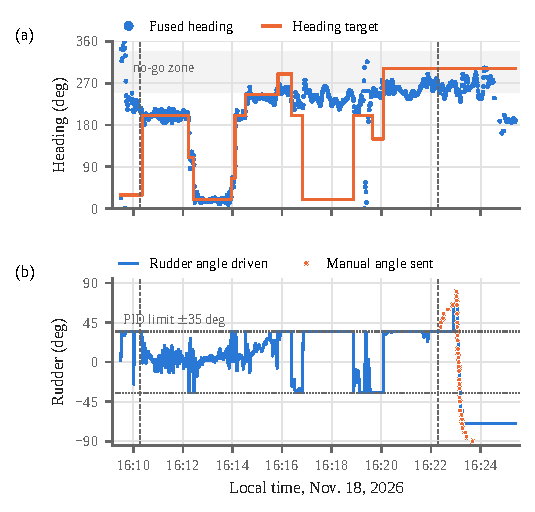
\includegraphics[width=\columnwidth]{field_heading}
\caption{Field test heading control, from launch. (a) Fused heading and heading
PID target; the shaded band is the no-go zone around the
\SI{294}{\degree} wind. (b) Rudder angle driven by the boat, with the PID's
$\pm\SI{35}{\degree}$ limit, and the manual angles sent during the final
sweep. Dashed lines mark the switch to semi rudder (16:10:16) and to manual
rudder (16:22:18).}
\label{fig:field_heading}
\end{figure}

\begin{figure}[!t]
\centering
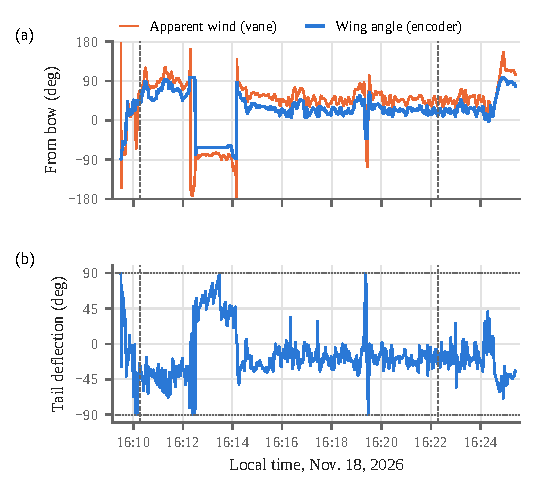
\includegraphics[width=\columnwidth]{field_sail}
\caption{Field test sail control. (a) Apparent wind angle from the vane and
wing angle from the AS5600 encoder, both relative to the bow; the gap between
them is the angle of attack. (b) Tail deflection commanded by the sail PID,
with its $\pm\SI{90}{\degree}$ limits. Dashed lines mark mode changes as in
Fig.~\ref{fig:field_heading}.}
\label{fig:field_sail}
\end{figure}

\paragraph*{Sail control}
Fig.~\ref{fig:field_sail} shows the wing angle following the apparent wind
with an offset, which is the angle of attack. Telemetry does not carry the
sail planner's target, so the target was recomputed from the logged wind
angle with~\eqref{eq:lsp} and Table~\ref{tab:lsp}. In the auto-sail modes on
the water, the wing angle stayed within \SI{10}{\degree} of the target half of
the time and within \SI{23}{\degree} 90\% of the time. Part of that error
comes from the planner's \SI{3}{\degree} deadband and the vane's averaging
window. The median angle of attack was \SI{24}{\degree}, and the tail
reached its $\pm\SI{90}{\degree}$ limit only 2\% of the time, so the
self-trimming wing could be steered with tail authority to spare.

\paragraph*{Stability, radio, and power}
The median heel on the water was \SI{13}{\degree}, the 95th percentile
\SI{29}{\degree}, and the single largest \SI{60}{\degree} at about 16:19:20,
after which the boat righted itself (Fig.~\ref{fig:field_roll}(a)). Pitch
stayed within a few degrees. The ground station received 1296 telemetry
packets and missed 55 (4.1\%), counted from sequence-number gaps. Most losses
fell in the final \SI{90}{\second}, near the far shore
(Fig.~\ref{fig:field_roll}(b)). Of the 65 commands sent, 29 were confirmed, one was
correctly refused (a heading target sent while the rudder was in AUTO), and 8,
all in the final \SI{90}{\second}, were never acknowledged. The remaining 27
were superseded before their result could be reported. Telemetry carries only
the latest command's result once per second, while the manual rudder sweep
sent commands about every \SI{0.3}{\second}. The GPS tracked 10 to 12
satellites with a differential fix the whole time on the water. The pack fell
from \SI{15.97}{\volt} to \SI{15.77}{\volt} over \SI{22.5}{\minute}. The
individual cell readings, however, varied with a standard deviation of about
\SI{180}{\milli\volt}, against \SI{74}{\milli\volt} for the pack, because
subtracting adjacent taps adds their noise.

\begin{figure}[!t]
\centering
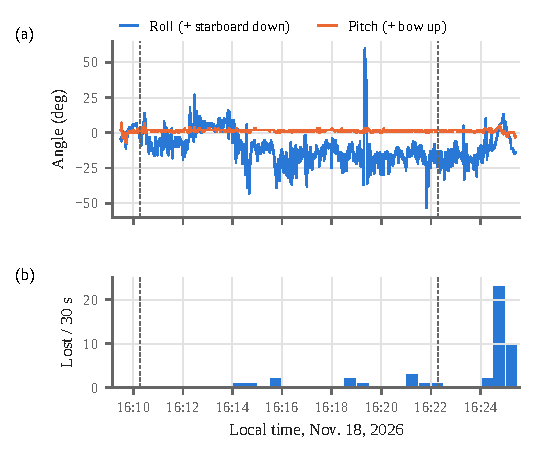
\includegraphics[width=\columnwidth]{field_roll_link}
\caption{Field test stability and radio link. (a) Roll (heel) and pitch from
the BNO055. (b) Telemetry packets lost in each 30-second bin, counted from
sequence-number gaps.}
\label{fig:field_roll}
\end{figure}

\begin{table}[!t]
\caption{Test Plan and Results}
\label{tab:tests}
\centering
\footnotesize
\begin{tabular}{@{}p{0.27\columnwidth}p{0.31\columnwidth}p{0.3\columnwidth}@{}}
\toprule
Test & Pass criterion & Result \\
\midrule
Navigation unit tests & All checks pass & 1275 of 1275 pass (\texttt{ltp} branch) \\
Firmware in the loop & Holds sail target in simulated gusts & Pass \\
Dummy telemetry & Ground station decodes every field & Pass \\
Hull leak test & No water inside after the field test & Pass \\
Float and trim & Level at design waterline & Pass \\
Radio link on water & Telemetry delivered to the far shore & 95.9\% of packets to \SI{228}{\meter} from launch \\
Sail loop & Wing angle follows planner target & Median error \SI{10}{\degree}, 90th percentile \SI{23}{\degree} \\
Manual rudder & Rudder follows ground-station angle & Swept $+80$ to $-70$ deg on command \\
Heading hold & Holds reachable targets & MAE 3.8--\SI{8.2}{\degree} at $\geq$\SI{49}{\degree} off wind \\
Turn through the wind & Reaches a target across the wind & Fail: stalled in irons; needs the tack planner \\
Waypoint course & All waypoints reached & Untested \\
Endurance & ~5-6 hours on one charge & \SI{0.2}{\volt} drop in \SI{22.5}{\minute}; full run untested \\
\bottomrule
\end{tabular}
\end{table}

\subsection{Demonstration}
The final demonstration is autonomous navigation of a waypoint route,
recorded on open water and shown by video at Demo Day.
